\section{V19}
\subsection{Typische Konzepte der Genexpressions-Präprozessierung}
\textbf{Motivation}\\
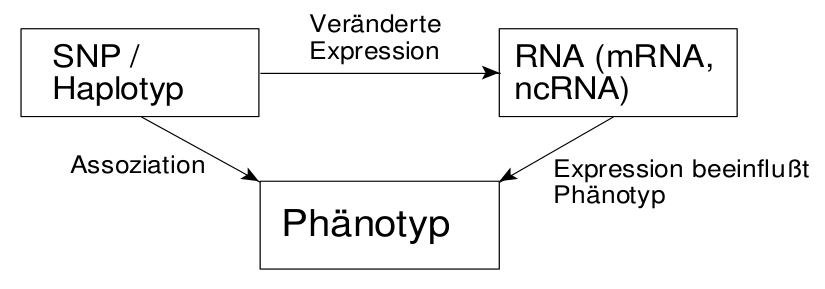
\includegraphics[width=1.00\textwidth]{lectures/V19/pix/pic1.png}
Genotyp-Phänotyp Assoziationen ergänzt durch funktionelle Analysen (z.B. Genotyp-Expression oder Expression-Phänotyp Korrelationen) ergeben Hinweise auf Pathomechanismen.
\\\\
\textbf{Prozessierung:}
\begin{itemize}
	\item RNA Extraktion
	\item RNA Aufreinigung / Fällung
	\item Sondensynthese / Hybridisierung / Scan
	\item Datenpräprozessierung (Normalisierung, Varianzstabilisierung, Filterungen, Adjustierungen) $\rightarrow$ Ziel: vertrauenswürdige Daten
	\item Datenanalyse
\end{itemize}

\textbf{Typische Designfalle}
\begin{itemize}
	\item Wenn bei einer Fall-Kontroll-Studie die Fälle und Kontrollen in verschiedenen Batches laufen, hat man hinterher kaum eine Chance, Batcheffekte von den interessanten Kontrasten zu unterscheiden
	\item Ideal ist eine Balancierung der Fälle und Kontrollen
	\item Eine gleichmäßige Verteilung ist auch ok
	\item Deshalb ist es wichtig, den Meßprozeß bereits aus Sicht einer späteren Auswertung zu beeinflussen
\end{itemize}

\newpage
\textbf{Vergleich verschiedener Normalisierungs- und Varianzstabilisierungsmethoden}
\begin{itemize}
	\item \textbf{Hintergrundkorrektur:} Korrektur der Kontraste innerhalb eines Arrays
	\item \textbf{Normalisierung:} Angleichung der Intensitäten unterschiedlicher Arrays
	\item \textbf{Varianzstabilisierung:} Angleichung der Streuung unterschiedlicher Transkripte
\end{itemize}

\textcolor{blue}{Bestes Vorgehen hängt von Technologie und Frage ab}
\\\\
\textbf{Präprozessierung Illumina HT12v4 (Beispiel)}
\begin{enumerate}
	\item \textbf{Ausgangspunkt:} Genexpressionsintensitäten von 47.000 Sonden
	\item \textbf{Individuenfilter 1:} Individuen mit geringer genomweiter Genexpression
	\item \textbf{Transkriptfilter 1:} Signal-to-noise Filter
	\item \textbf{Reduktion technischer Artefakte 1:} Quantilnormalisierung, Varianzstabilisierung (log2-Transformation)
	\item \textbf{Individuenfilter 2:} Individuen mit atypischen technischen Qualitätsparametern
	\item \textbf{Reduktion technischer Artefakte 2:} Reduktion von Batcheffekten mittels Empirical Bayes Methoden
	\item \textbf{Individuenfilter 3:} Ausreißer bezüglich Genexpression
	\item \textbf{Reduktion biologischer Artefakte 3:} Residualisierung bezüglich Alter, Geschlecht, Blutwerte (Mo, Ly, Gra, Ret), Rauchen, ggf. unbekannter Batch-Effekte
\end{enumerate}

\textcolor{blue}{Resultat der Präprozessierung: 28.000 Sonden}
\\\\
\textbf{Was heißt „exprimiert“?}
\begin{itemize}
	\item Man prüft Intensität des Transkripts im Vergleich mit Leersonden (Sequenzen die im Genom keine Entsprechung haben, d.h. nicht hybridisieren sollten)
	\item Detection p-value = Anteil Leersonden mit höherer Expression (kein eigentlicher p-Wert)
	\item 5\% (andere verwenden 1\%) als cut-off zur Entscheidung „exprimiert“ vs. „nichtexprimiert“
	\item Stark gewebsabhängig
	\item Über alle Gene und Individuen hinweg sind ca. 60\% der Gene / Transkripte in Blut (PBMCs) exprimiert
\end{itemize}

\subsection{Typische Filter / Probleme}
\textbf{Individuenfilter 1}
\begin{itemize}
	\item Individuen mit atypischer Zahl exprimierter Gene
\end{itemize}

\textbf{Transkriptfilter 1}
\begin{itemize}
	\item Transkript wird gefiltert, wenn z.B. in weniger als 5\% der Individuen exprimiert
	\item Z.B. im Blut: Von den Genen sind ca. 60\% in mehr als 5\% der Individuen transkribiert, also gültig bzgl. Transkriptfilter 1
\end{itemize}

\textbf{Quantilnormalisierung}
\begin{itemize}
	\item Idee: Bilde Quantile der Intensitäten aufeinander ab um Intensitätsprofile anzugleichen
\end{itemize}

\textbf{Reduktion technischer Artefakte 1}
\begin{itemize}
	\item QL = Quantilnormalisierung + log2-Transformation(Varianzstabilisierung)
	\item \textcolor{red}{Für was steht QL?}
\end{itemize}

\textbf{Individuenfilter 2}
\begin{itemize}
	\item Idee: Exkludiere Individuen mit atypischen Ergebnissen in speziellen Kontrollsonden
	\begin{itemize}
		\item Filtere Individuen mit Zu großem Mahalanobis-Abstand zum Mittelwert der internen Qualitätsparameter = atypische (schlechte) Qualität
		\item \textbf{Mahalanobis-Abstand:} Seien x,y Realisierungen einer multinominalen Normalverteilung mit Kovarianzmatrix S (in unserem Falle stellen die Qualitätsparameter für ein Sample eine solche Realisierung dar), so berechnet sich die Mahalanobisdistanz wie folgt:\\
$d(x,y)=\sqrt{(x-y)^T S^{-1}(x-y)}$ \textcolor{red}{Was ist T???}
	\end{itemize}
\end{itemize}

\textbf{Reduktion technischer Artefakte 2}
\begin{itemize}
	\item Batch-Effekte verursacht durch Meßprozeß (hauptsächlich Hybridisierung)
	\item Problem: Viele Batches geringer Größe $\rightarrow$ keine klassische Adjustierung möglich (Regression)
	\item Lösung: Empirical Bayes – Verfahren
\end{itemize}

\textbf{Individuenfilter 3}
\begin{itemize}
	\item Idee: Betrachte Genexpression als multivariaten Phänotyp,  Filtere Individuen mit zu großem Abstand vom Zentrum = atypisches Expressionsprofil
\end{itemize}

\textbf{Reduktion technischer Artefakte 3}
\begin{itemize}
	\item Adjustierung auf biologische Faktoren
\end{itemize}


\subsection{Konzepte für Anreicherungsanalysen}
Anreicherungsanalysen = Überrepräsentationsanalyse\\\\
Verwendet z.B. hypergeometrische Verteilung, um die Wahrscheinlichkeit zu bestimmen, in einer Anzahl von Versuchen (Vordergrund) eine bestimmte Anzahl Treffer in der Gesamtmenge (Hintergrund) zu erzielen\\\\
Wie groß ist die Wahrscheinlichkeit (p-Wert) dass genau 260 Gene (von 747) auf die Erkrankung abbildbar sind, gegeben dass 3005 dieser Gene im Hintergrund sind (13,101 genes)? $\rightarrow$ \textbf{Hypergeometrischer Test / Fisher’s exakter Test}

\textbf{Limitationen}
\begin{itemize}
	\item Reihenfolge der Assoziationsstärke der Top-Hits wird nicht beachtet
	\item Richtung der Effekte wird nicht beachtet
	\item Richtung von Gen-Gen-Interaktionen wird nicht beachtet
	\item Verschiedene Cut-offs für Genlisten erzeugen unterschiedliche Ergebnisse
	\item Überlappungen zwischen Pathways werden nicht berücksichtigt (Unabhängigkeit der Tests ist nicht gegeben)
	\item Signifikanz wird tendenziell überschätzt, wenn ein Gen in vielen Pathways liegt
	\item \textcolor{red}{P-Werte aus diesen Analysen sollten eher als qualitative Orientierung dienen und keinesfalls überbewertet werden}
\end{itemize}

\textbf{Functional Class Scoring: GSEA}
\begin{itemize}
	\item GSEA: gene set enrichment analysis
	\item Ordnung der Gene nach Signifikanz. Liegen Gene eines Subsets tendenziell weiter vorn in der Liste?
	\item Signifikanztest per Komolgornov Smirnov/Permutation
	\item Vorteile: 
	\begin{itemize}
		\item Benötigen keinen Cutoff der Topliste
		\item Sensitiv zu kleineren Effekten, wenn Sie alle im gleichen Pathway liegen
	\end{itemize}
	\item Limitationen
	\begin{itemize}
		\item Überlappungen zwischen Pathways werden nicht beachtet
		\item Richtung des Zusammenhangs wird nicht beachtet
		\item Richtung von Gen-Gen-Interaktionen wird nicht beachtet
	\end{itemize}
\end{itemize}

\textbf{Pathway Topologie}\\
Bewertet nicht nur Vorkommen des Gens im Pathway, sondern auch Rolle des Gens: Beeinflusst es zentral mehrere Gene (a) oder weniger (b) erzeugen verschiedene Ergebnisse \textcolor{red}{Wie muss ich das lesen???}

\textbf{Limitationen}
\begin{itemize}
	\item Überlappungen zwischen Pathways werden nicht beachtet
	\item Topologische Annotationen oft nur eingeschränkt verfügbar
	\item Verlässlichkeit des eingepreisten Wissens nicht berücksichtigt
	\item Verschiedene Cut-offs erzeugen verschiedene Ergebnisse
\end{itemize}